\documentclass[classical]{einfart}
\usepackage{ProjLib}
\usepackage{hologo}
\usepackage{graphicx} %插入图片的宏包
\usepackage{float} %设置图片浮动位置的宏包
\usepackage{subfigure} %插入多图时用子图显示的宏包
\usepackage{hyperref}

\UseLanguage{TC}
%%================================
%% Titles
%%================================
\let\LevelOneTitle\section
\let\LevelTwoTitle\subsection
\let\LevelThreeTitle\subsubsection

\providecommand{\tightlist}{%
  \setlength{\itemsep}{0pt}\setlength{\parskip}{0pt}}


\begin{document}

\setcounter{tocdepth}{2}
{\setstretch{1.07}\tableofcontents}

\newpage

\part{開發專案}

\section{高中}

\subsection{專題網頁競賽}

技術路線:Gulp.js、SASS、Markdown

Github: \url{https://github.com/junyussh/opentix}

\begin{figure}[H]
    \centering
    \subfigure[網頁界面]{\label{Fig.sub.1}
    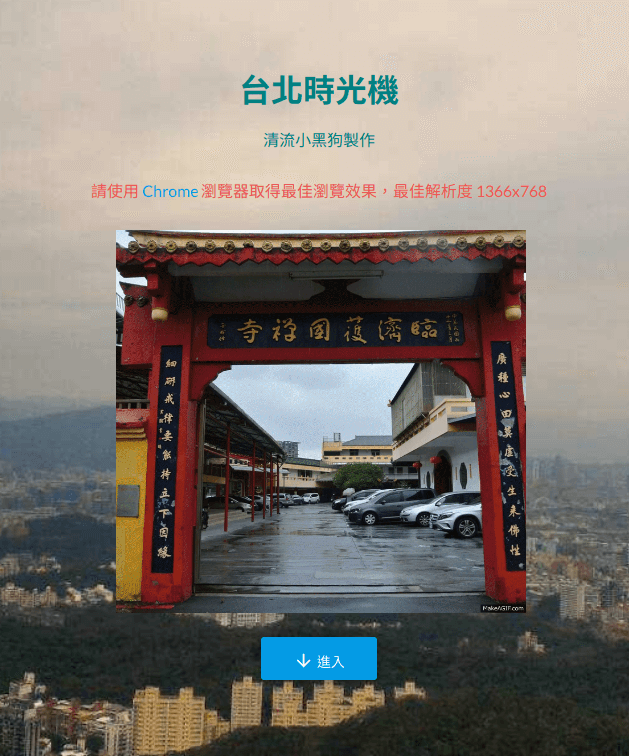
\includegraphics[width=0.45\textwidth]{images/html_contest.png}}
    \subfigure[獎狀]{\label{Fig.sub.1}
    \includegraphics[width=0.45\textwidth]{images/網頁比賽}}
    \caption{專題網頁競賽}
\end{figure}

高一時前參加台北市專題網頁競賽的作品,這算是我接觸前端的一個較大轉捩點,用了
Gulp.js 這類前端自動化構建工具,當時是叫同學先用 Markdown
編輯內容,界面設計我是參考流行的 Material Design,用\textbf{手刻的
CSS,沒有用前端框架},然後寫一個簡單的界面框架。內容的部份我用 Gulp.js
的 Markdown 套件,再寫個 Node.js 腳本來產生多個
HTML,然後複製到之前的前端框架,再手動連結其他網頁。當時的作品還比較土法煉鋼,不過我們是班上唯一獲獎的組,獲得了佳作,網頁的部份全部我寫的,內容撰寫是其他同學負責的。

\subsection{Opentix}

技術路線:Node.js、JWT、MongoDB

Github: \url{https://github.com/junyussh/opentix}

這是高二資訊班成果發表會寫的作品,想做一個開源版的 KKTIX
訂票系統,語言我選擇用當時流行的 Node.js 寫,這也是第一次用 Node.js
寫後端,為了開發出接近現代流行的架構,還特地去網路上研究了前後端分離架構,以及
RESTful API、JWT 的概念。資料庫用了 MongoDB,以前都是用
MySQL,但我想到樹狀結構 MySQL 不好實現,於是選擇了 NoSQL 的
MongoDB,還去研究各種資料查詢的可行性。由於當時對 Node.js
還不熟,程式碼模組化沒做好,導致後面功能開發困難,也算是土法煉鋼的作品。雖然技術拙劣沒寫好,但有了相應的
Web 知識也讓我對之後開發專案有了相當大的幫助。

\subsection{校園氣象站}

硬體:Raspberry Pi、Ardunio 前端:Gulp.js、Susy 2 後端:Django

Github: \url{https://github.com/oxygen-TW/Campus-Weather-Service}

\begin{figure}[H]
    \centering
    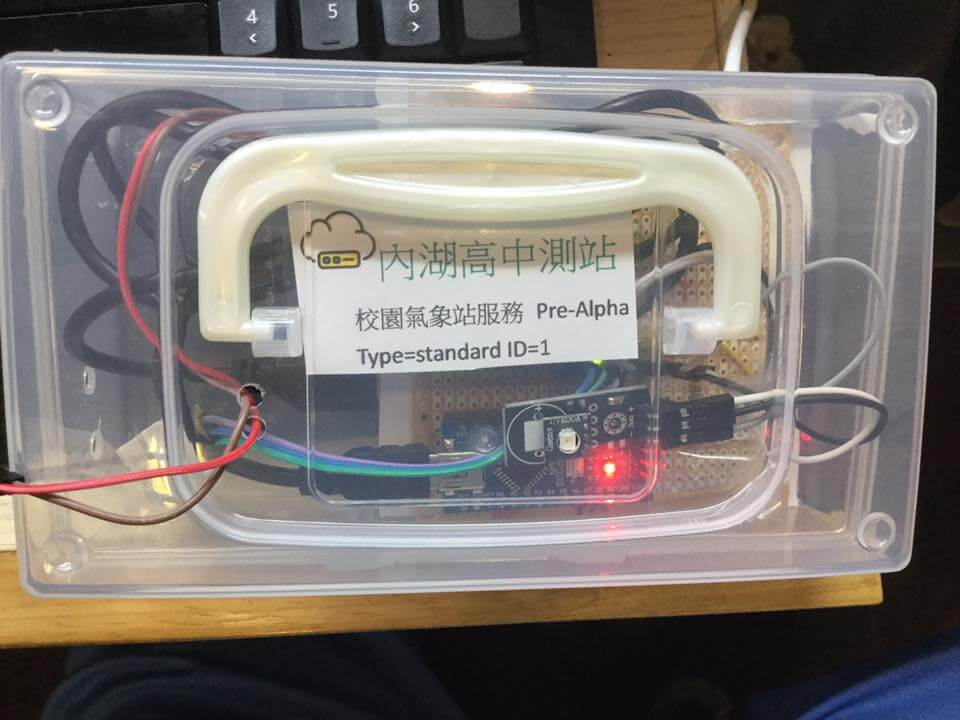
\includegraphics[width=0.7\textwidth]{images/weather_box.jpg}
    \caption{校園氣象站的氣象盒子}
\end{figure}

這是和擅長開發的班上同學一起開發的專案,當時是資訊研究社的指導老師把我們組織在一起開發的,也算是興趣使然的專案,當時目標是希望台北的高中都能用上我們這套系統。我負責開發前端的部份,另外兩位同學開發硬體和後端。參加了\textbf{校內科展生活與應用科學組
優等獎},也參加中學生獎助計畫獲得決審機會。在參與過程中,老師將機房閒置的主機借給我們使用,讓我們有了真實環境可以管理
Linux
伺服器,還曾請公假到外校去宣講計畫、部署設備,從中我學習到寶貴的\textbf{開發經驗和
Linux 伺服器管理經驗},也了解到開發一套產品是件多麼不容易的事。

\subsection{校園氣象站界面}

技術路線:Gulp.js、SASS、Susy2

Github: \url{https://github.com/junyussh/weather-view}

\begin{figure}[H]
    \centering
    \includegraphics[width=0.7\textwidth]{images/校園氣象站服務.png}
    \caption{校園氣象站服務首頁}
\end{figure}

這次的前端依舊採用了土法煉鋼的方法,沒有用前端框架,連 CSS
網格系統也是用 Susy2
自動產生的,主要目標是讓後端的數據能夠呈現在前端上,本來想說用純 JS
寫,後面才意識到需要用 Vue
這種框架才能方便綁定前後端,但來不及學,功能也就不完全了,主要還是在研究界面的設計。

\subsection{Weather Station API}

技術路線:Node.js、Express、JWT、Redis

Github: \url{https://github.com/junyussh/opentix}

這個專案誕生純屬意外,後端工程師遲遲不給 API
接口,於是用了週末兩天自己開幹。有了前面 Opentix
的慘痛經驗,這次我學會了用 Express 框架來開發 API
系統,大量減少我的程式碼,還參考了別人的範例原始碼來優化程式結構,這次算是真正意義的模組化了,從中也學會了
Redis 的使用和資料結構。

\section{大學}

\subsection{MumiChat}

技術路線:Qt、Golang、gin、WebSocket

後端 Github: \url{https://github.com/junyussh/MumiChat-server}\\
前端 Github: \url{https://github.com/junyussh/MumiChat-Client}

\begin{figure}[H]
    \centering
    \subfigure[起始界面]{\label{Fig.sub.1}
    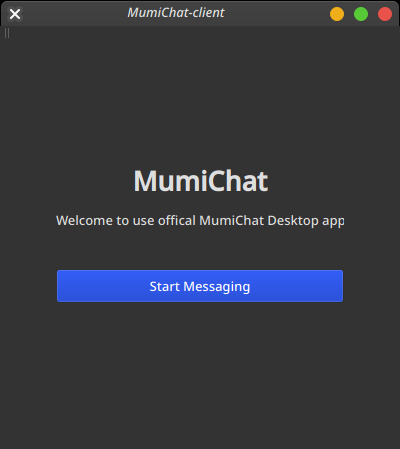
\includegraphics[width=0.7\textwidth]{images/mumichat_welcome.png}}
    \subfigure[聊天界面]{\label{Fig.sub.1}
    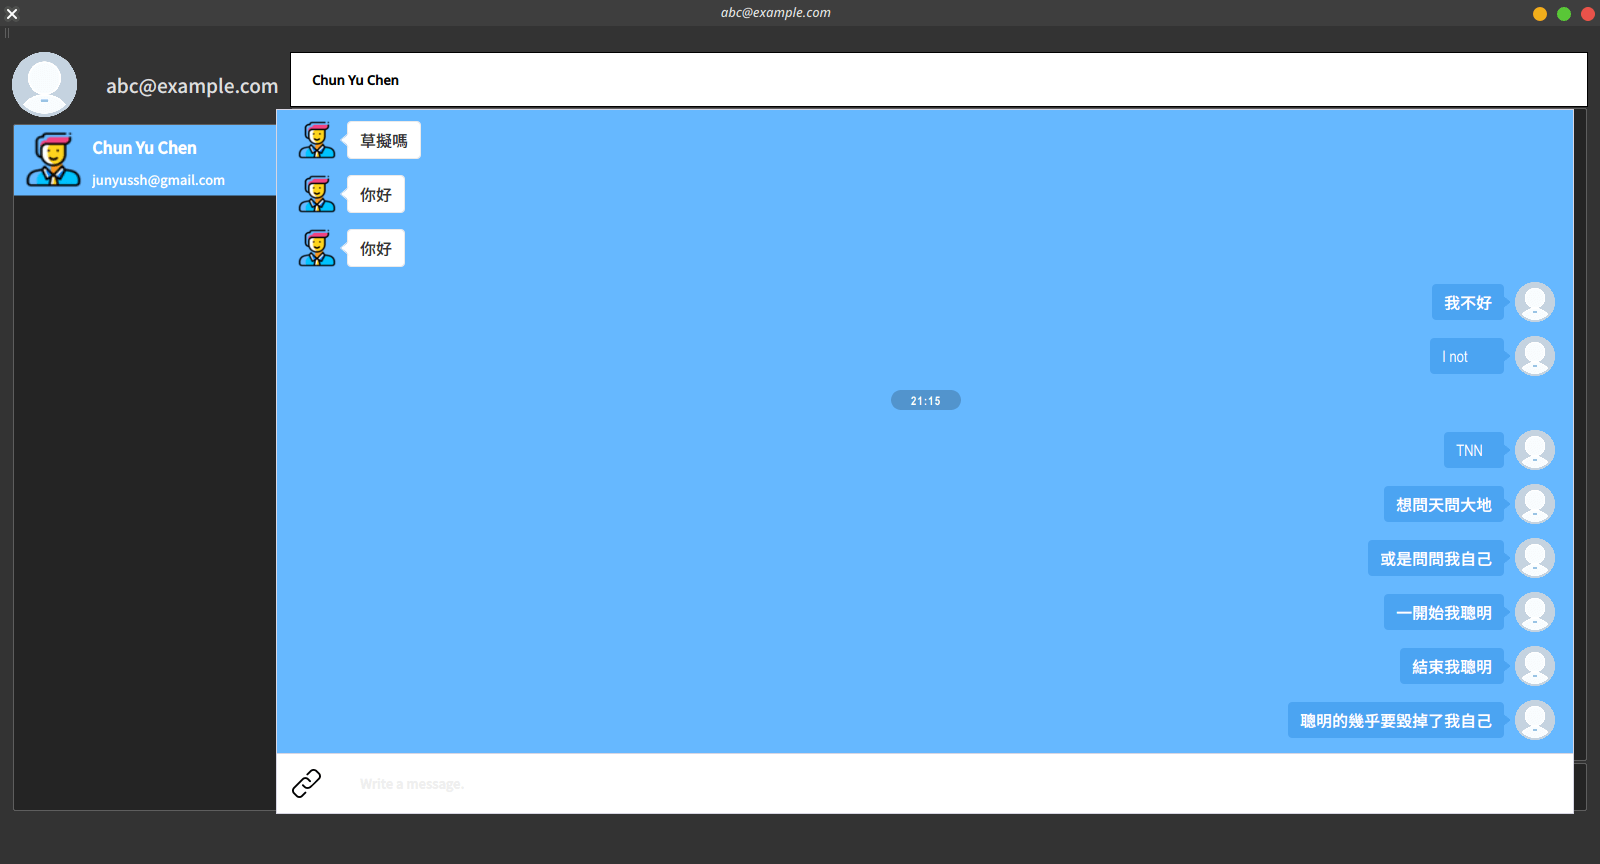
\includegraphics[width=0.7\textwidth]{images/mumichat_chat.png}}
    \caption{MumiChat 畫面展示}
\end{figure}

大一實訓時開發的簡單聊天工具,資料結構與接口皆為原創,前端圖形界面用 Qt
開發,當時為了挑戰自己,後端核心選擇熱門的 Golang 編寫,因為 Golang
適合開發網路應用且可以編譯成二進制,除了方便部署效能也較佳,由於是初次撰寫
Golang,開發過程中在網路上查了不少資料,熬夜多日完成的鉅作,使用
WebSocket 協定通訊。本作品屬於個人獨立開發,最終獲得實訓三等獎。

\subsection{JPetstore}

技術路線:Spring Boot、Spring Security、Swagger、MyBatis、Nuxt.js

Github: \url{https://github.com/junyussh/New-JPetstore}

\begin{figure}[H]
    \centering
    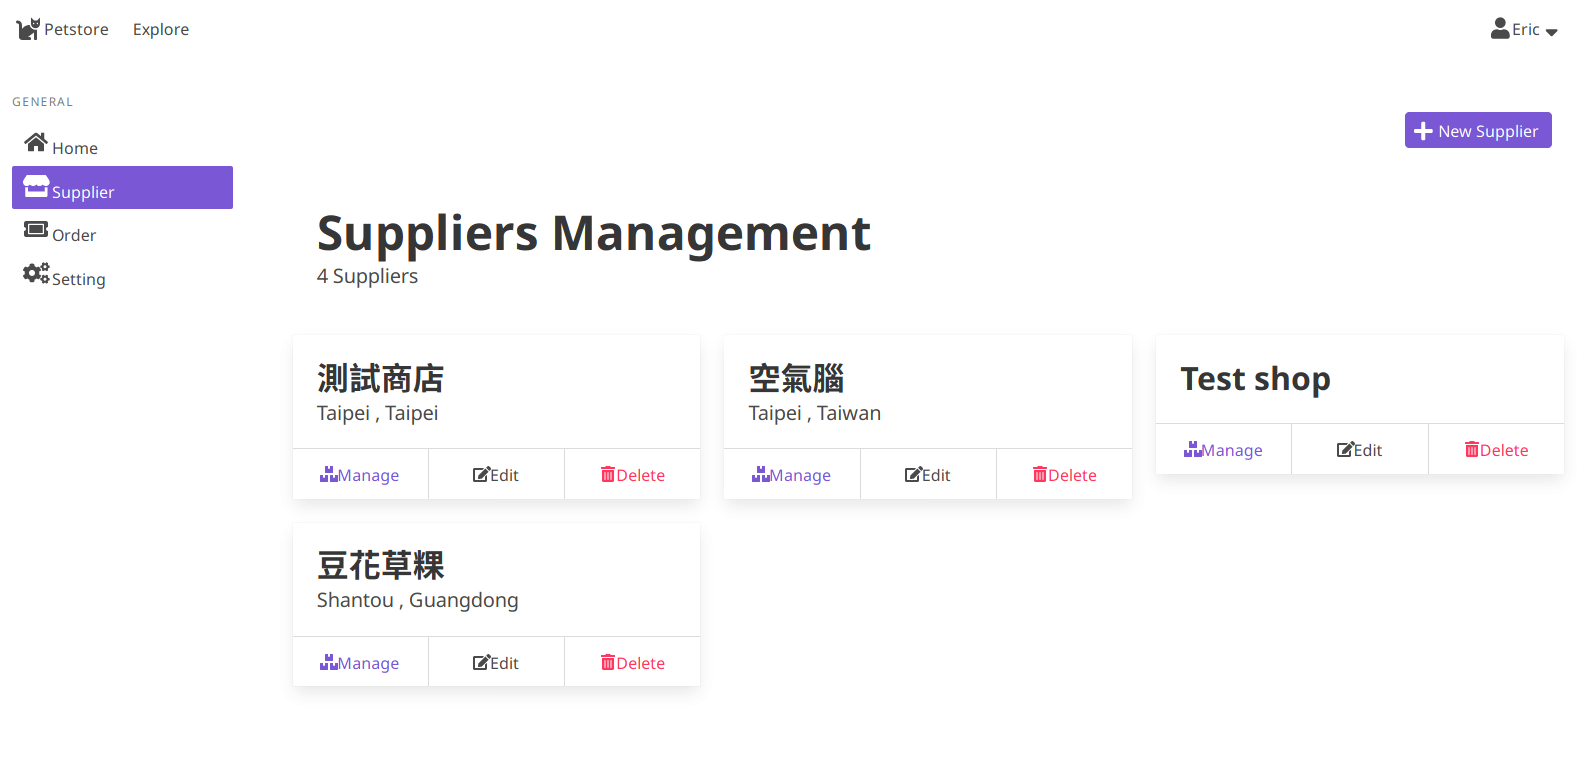
\includegraphics[width=0.7\textwidth]{images/petstore.png}
    \caption{寵物商店頁面}
\end{figure}

大二軟件開發架構的課程作業,為小組開發,用 Spring Boot
框架開發的多賣家寵物商店,原先架構是用同組同學上學期的作業 Spring
MVC+MyBatis+Thymeleaf,但是用的是模板引擎,耦合性太高,加上原先資料表過多冗餘欄位,於是我決定構造改革,改為前後端分離結構
Spring Boot+Swagger+MyBatis,使用 Spring Security
進行權限控制,資料表、接口、架構、前端界面都由我設計,前後端也是我主導開發,不眠不休寫了一星期,也讓我的組員在作業上獲得了高分。這次專案中,我的工作佔
70\% 左右。

\subsection{UniFit}

技術路線:Spring Boot、Spring Security、Swagger、MyBatis、Nuxt.js

前端 Github: \url{https://github.com/junyussh/UniFit_frontend}


\begin{figure}[H]
    \centering
    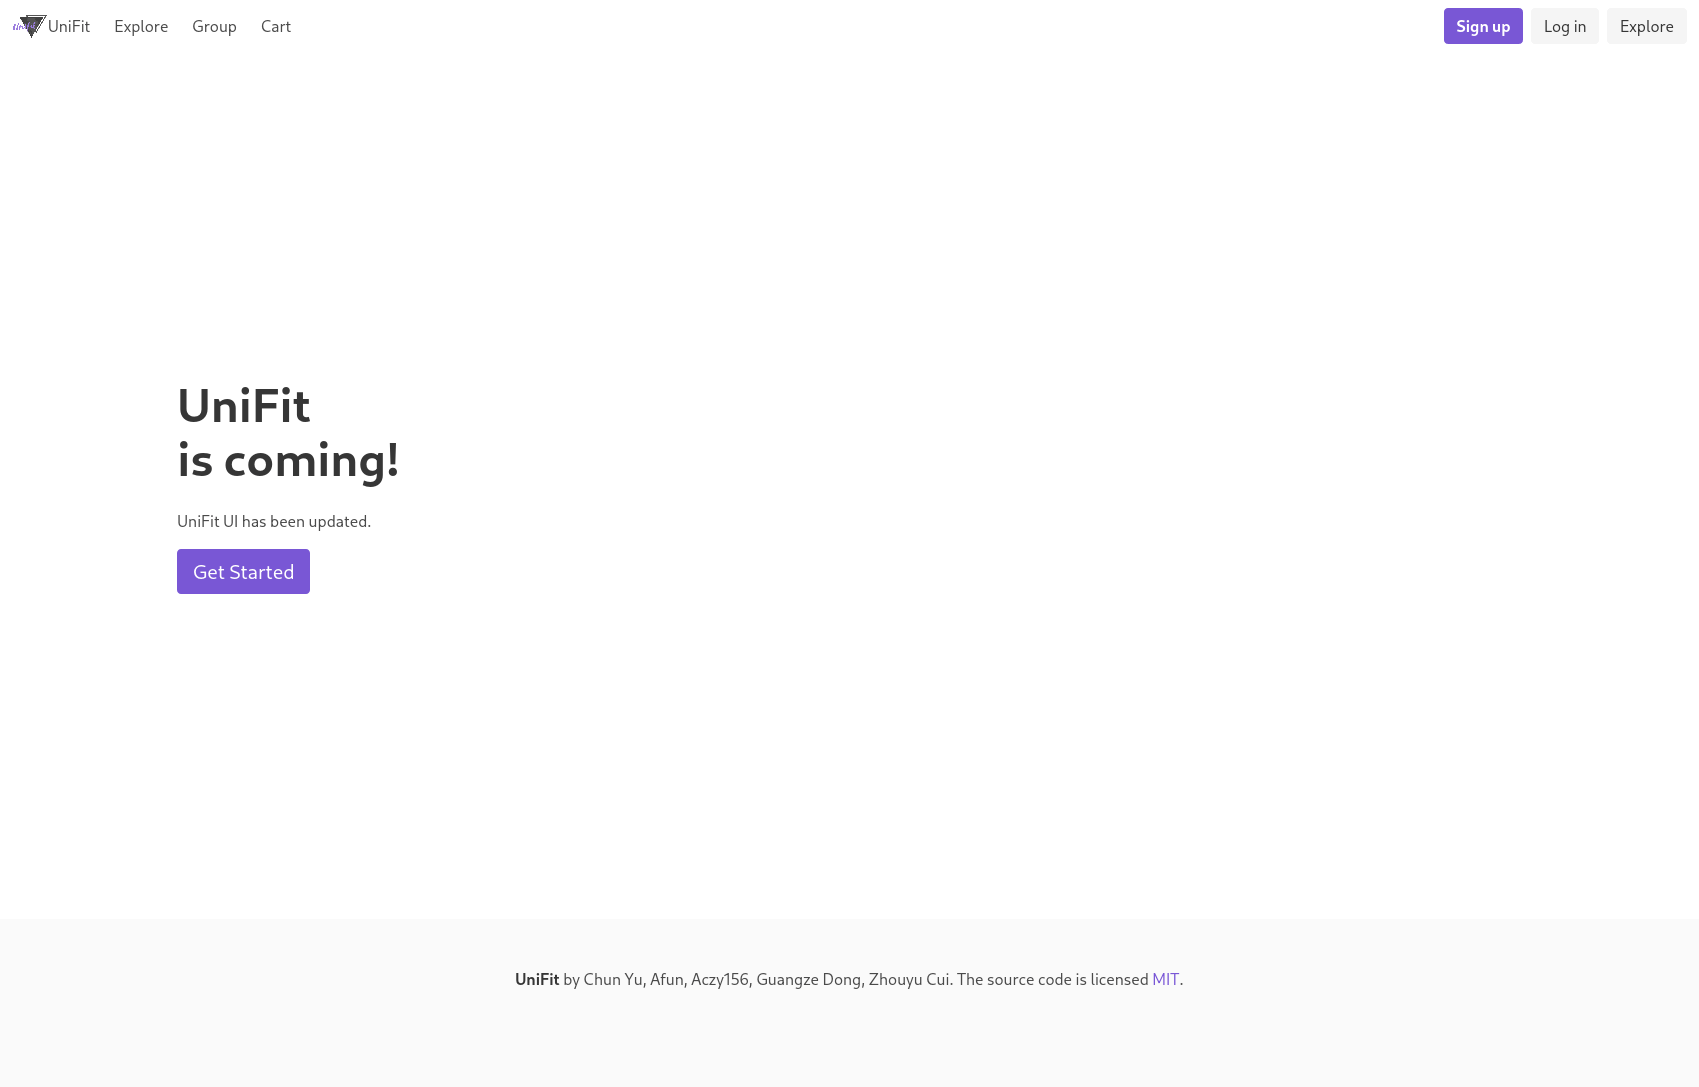
\includegraphics[width=0.7\textwidth]{images/unifit.png}
    \caption{UniFit 首頁}
\end{figure}

大二暑假實訓小組開發的團購系統,與 JPetstore
採用相同架構設計,多添加了幾張表實現了團購系統,團隊分工採用 Trello
進行任務管理、Git 版本控制、HackMD
上共筆開發標準,由於採用標準開發流程、完整的功能展示、漂亮的界面、足夠的工作量,讓我們組在班上獲得最高分,我的工作量大概佔
30\% 左右。

\subsection{爬取 Github 中國用戶貢獻情形}

技術路線:Python、GraphQL、Pandas

Github: \url{https://github.com/junyussh/GithubChinaUserFetch}

\begin{figure}[H]
    \centering
    \subfigure[用戶所有倉庫平均 Fork 數]{\label{Fig.sub.1}
    \includegraphics[width=0.45\textwidth]{images/用户所有仓库的平均fork数.png}}
    \subfigure[用戶所有倉庫總 Fork 數]{\label{Fig.sub.1}
    \includegraphics[width=0.45\textwidth]{images/用户所有仓库的总fork数.png}}
    \caption{數據分析}
\end{figure}

大三機器學習與數據挖掘課程實驗,我選擇研究中國 Github 用戶的使用情況,利用 Github API 採集了用戶的 followers 數量、倉庫的 Stars, Forks 數、用戶所屬組織、倉庫語言、Topics 等數據來分析,
因為 Github 的 HTTP API 有過多不需要的欄位,直接抓取會太慢,而且我要獲取的數據又具有一定關聯性,而 GraphQL 可以使用特定查詢語言進行嵌套查詢,所以使用 GraphQL 查詢是最佳解決方案。這次專案我主要負責數據
的爬取腳本撰寫。

\subsection{LotsDrawer}

技術路線:Flutter

Github: \url{https://github.com/oxygen-TW/LotsDrawer}

% \begin{figure}[H]
%     \centering
%     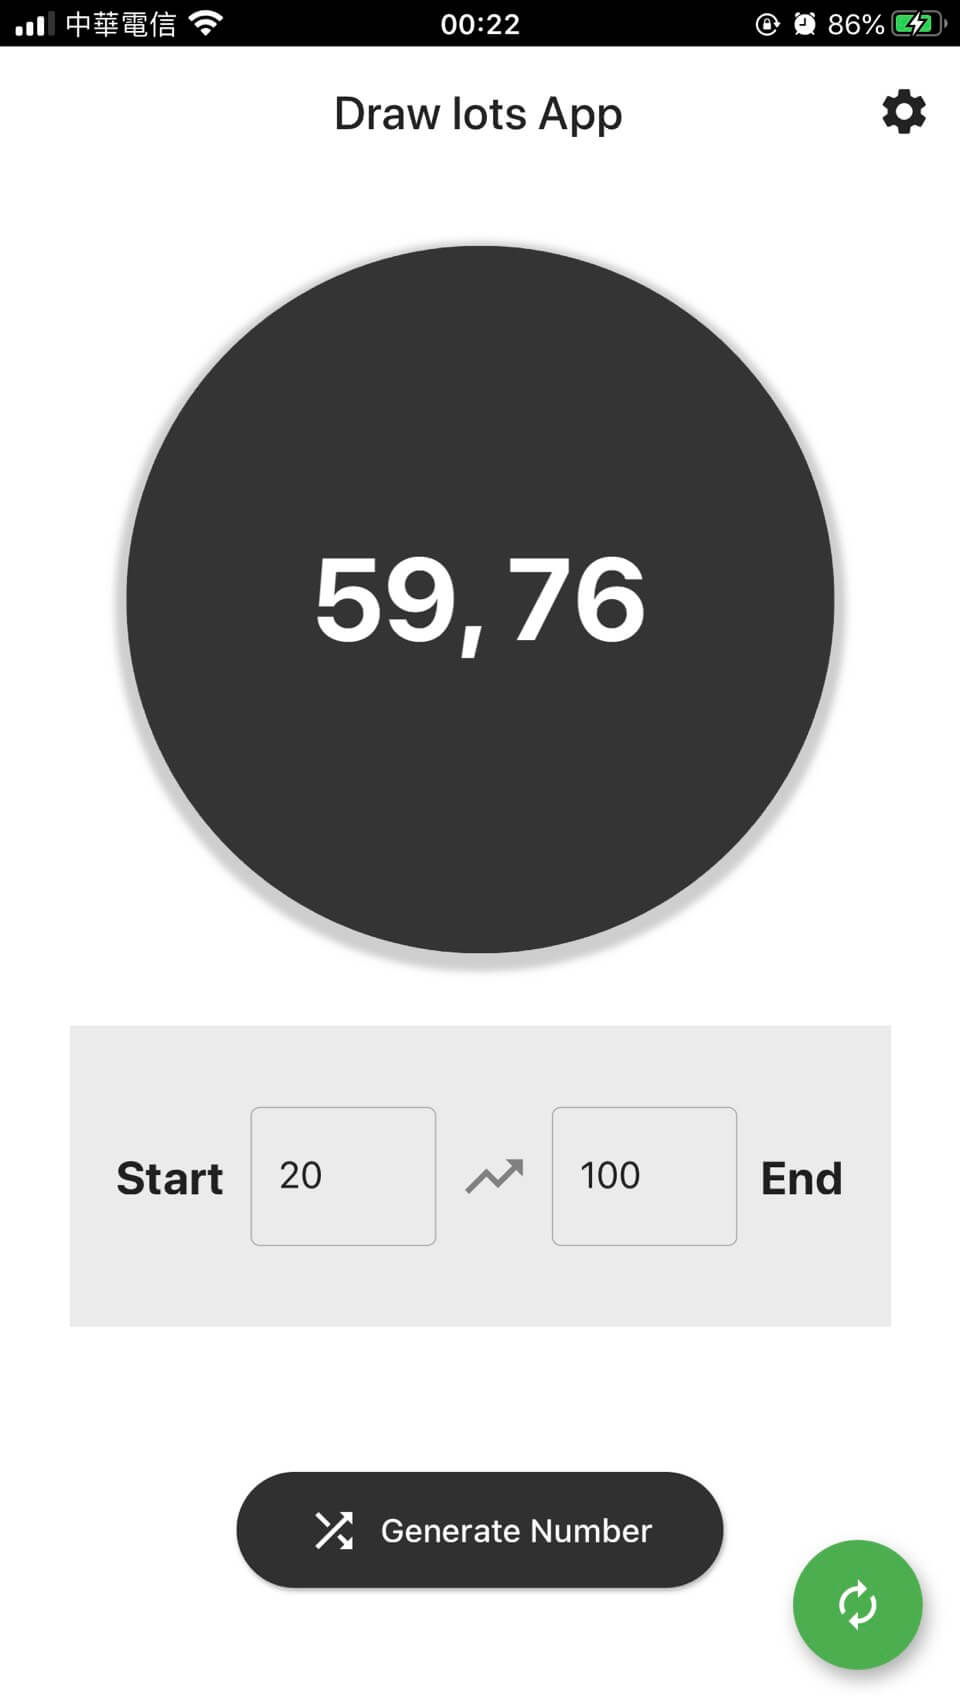
\includegraphics[width=0.7\textwidth]{images/lotsofdrawer.jpg}
%     \caption{APP 畫面}
% \end{figure}
\begin{figure}[H]
    \centering
    \subfigure[抽籤界面]{\label{Fig.sub.1}
    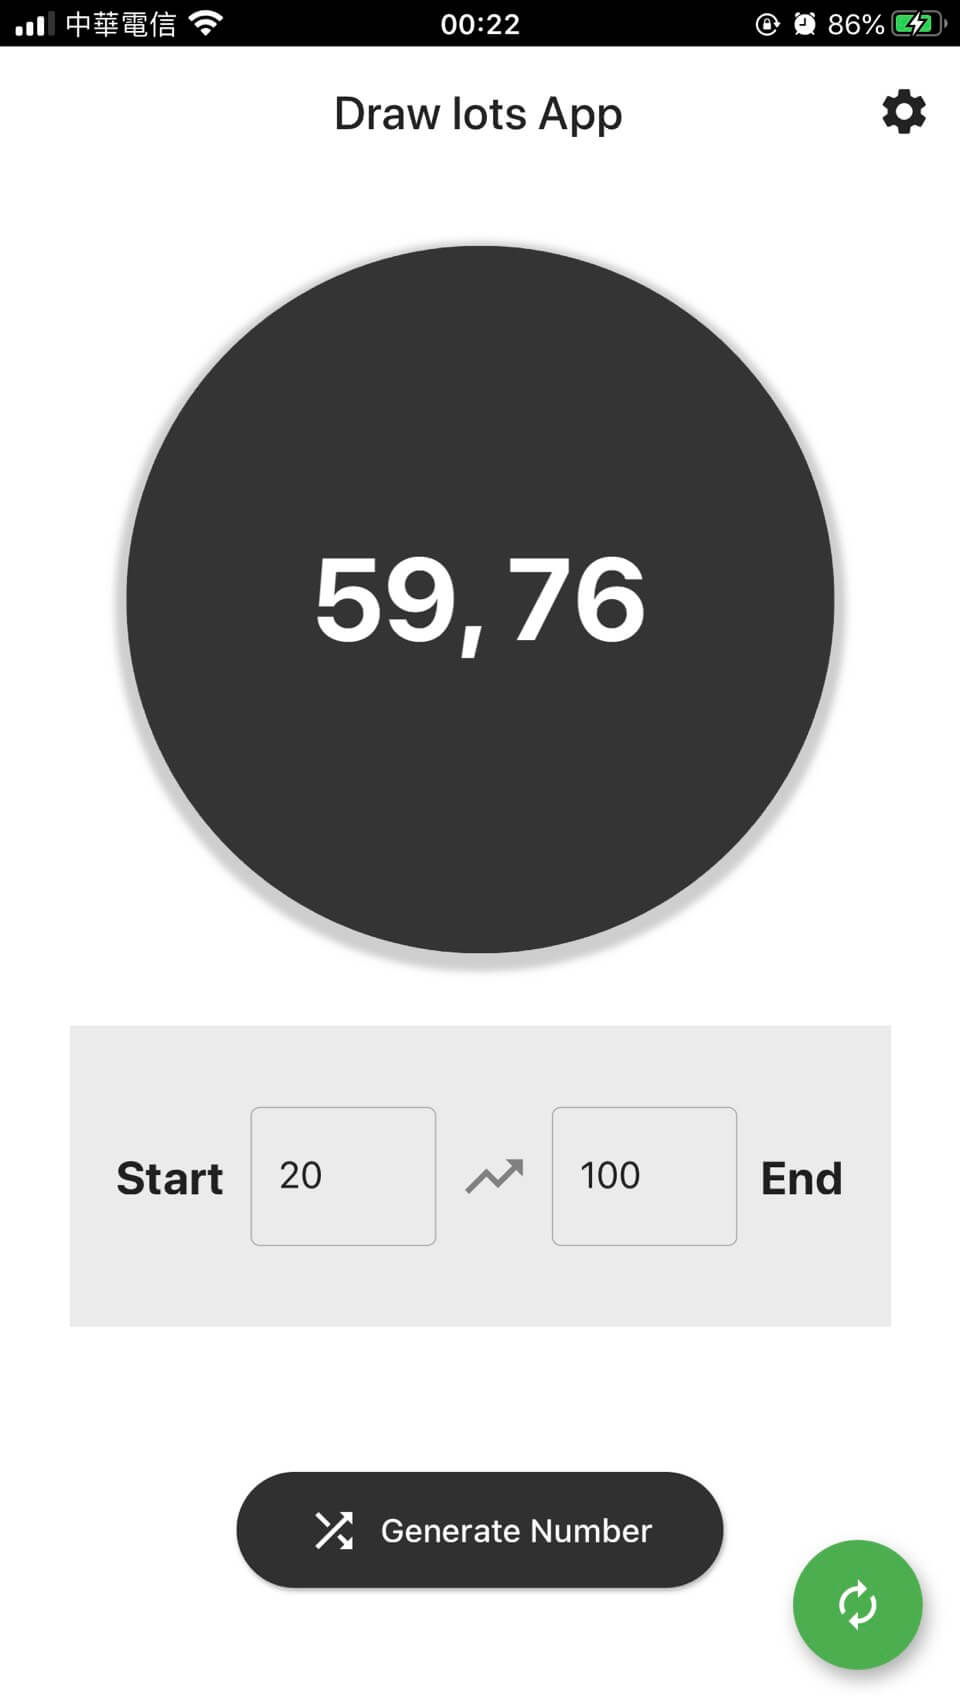
\includegraphics[width=0.45\textwidth]{images/lotsofdrawer.jpg}}
    \subfigure[設定界面]{\label{Fig.sub.1}
    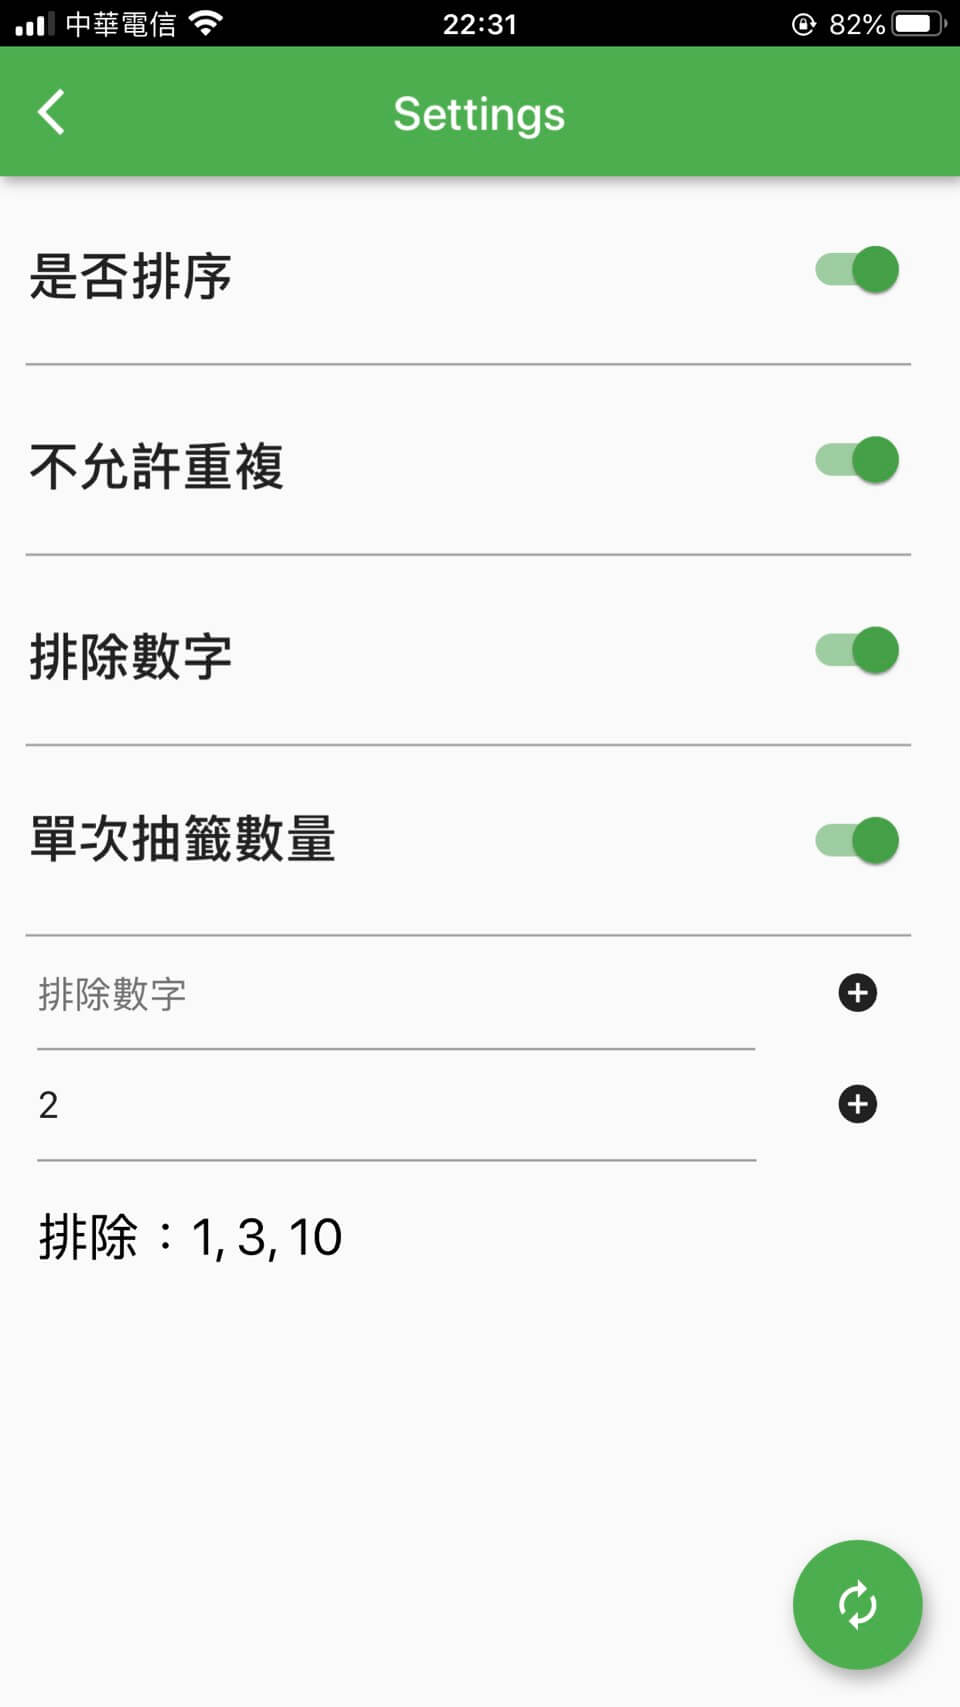
\includegraphics[width=0.45\textwidth]{images/lotsofdrawer_setting.jpg}}
    \caption{APP 畫面展示}
\end{figure}

暑假上完 Google DSC 線上課程後和高中同學共同開發的開源小專案,用 Flutter
寫的簡單抽籤 APP,並在 Google Play 上架,我負責界面設計的部份,曾獲得
Google DSC 評優,我大概佔 50\% 的工作量。

\part{工作經驗}

\section{聯立達科技 智慧社區雲}

\begin{figure}[H]
    \centering
    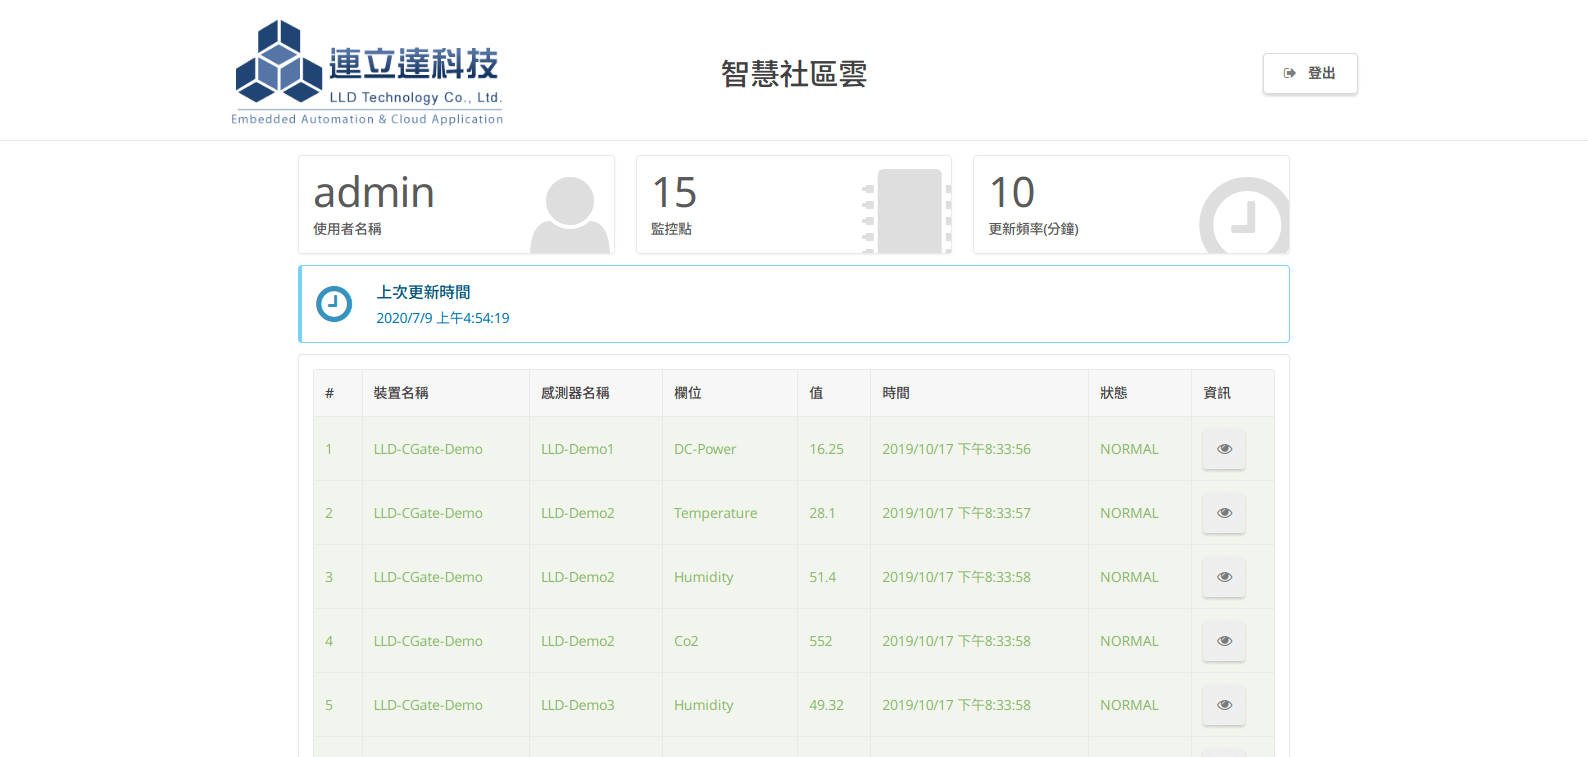
\includegraphics[width=0.7\textwidth]{images/iot_cloud.png}
    \caption{智慧社區雲管理畫面}
\end{figure}

因為學測就錄取大學了,高中畢業後較閒,便被父親介紹去他產學合作的公司開發軟體賺外快。該公司主要業務是開發嵌入式系統,比較缺乏軟體工程師,於是希望我協助他們開發一個物聯網系統的
DEMO
用來推廣他們的嵌入式系統。前端後端都是我一個人開發對接,還接觸了底層一點的
Socket 通訊和 GPIO
控制,也了解到\textbf{完成一個產品的需要長時間的測試與多版本的迭代}才能做出一個初步可用的雛型。

\end{document}
